

\chapter{Testing}

\section{Variable DC load using MOSFET}
To test the efficiency of the demo boards, different tests like line regulation, load regulation etc have to be conducted. For line regulation, at a certain constant load, we should create a voltage values table and get the efficiency curve. For that, we need different values of resistance (load). Instead of using resistance, we could use a MOSFET for simulating various load conditions. Since we doesn’t need any higher loads to test the demo boards, a circuit that simulate a load precisely for values from 0 to 2A and with a precision of 0.01A will do the job.
\\ \\

The working of the circuit is simple. The MOSFET is controlled by voltage on its gate. Till the voltage between gate and source (Vgs) is not higher than a certain value called Vth, the MOSFET is disabled, so no current will be flowing between drain and source. After Vth, the MOSFET starts a current flow and the value of this current will get higher as Vgs increases till a certain value where the MOSFET is fully on. So, by varying the voltage at the gate we change the current flow and by that we can simulate the load value. 
\\ \\
\begin{figure}[h]
	\centering
	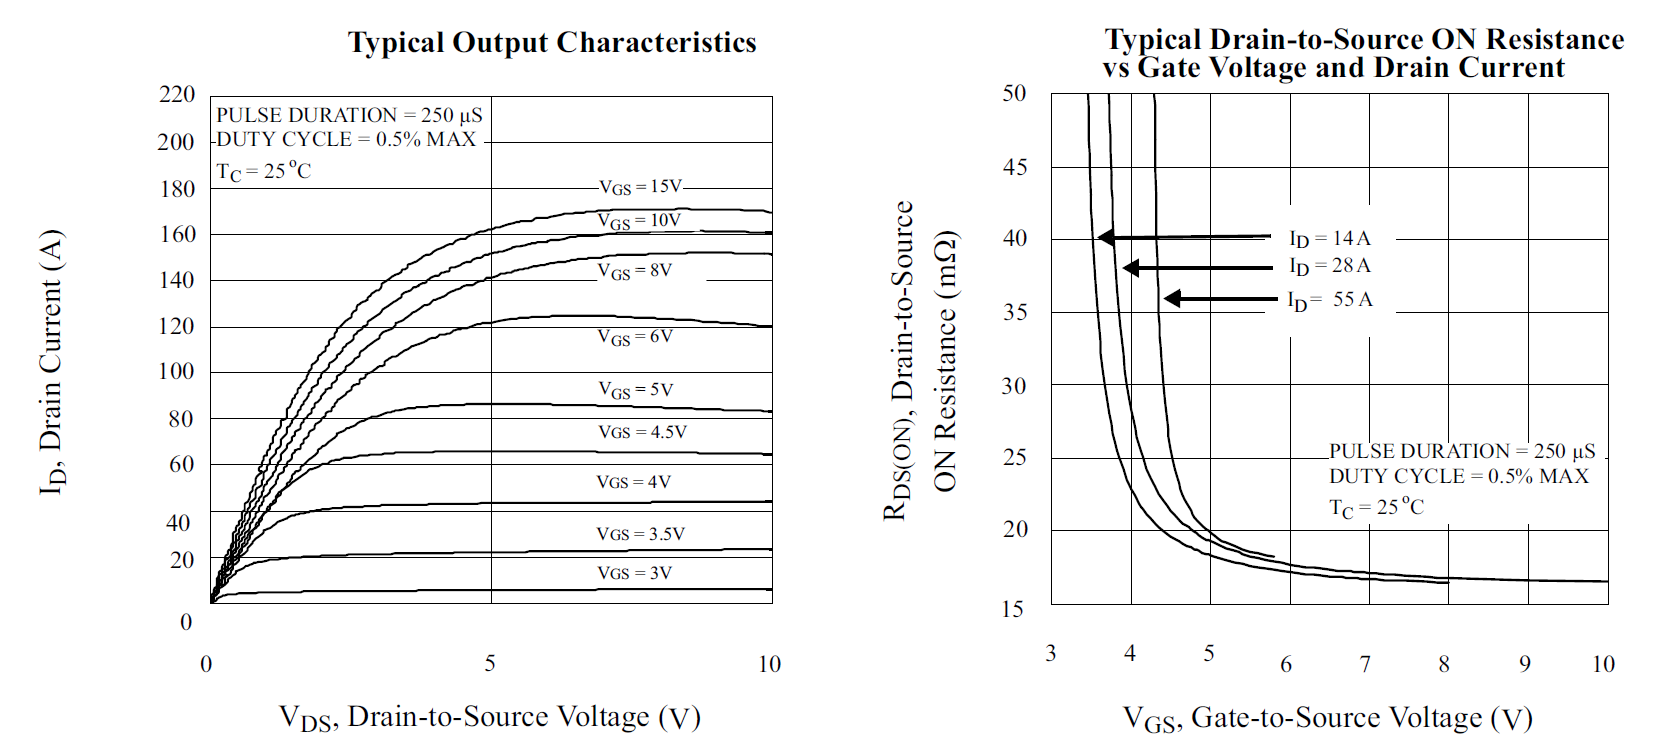
\includegraphics[width=\columnwidth]{IMGS/MosfetChara.jpg}
	\caption{Mosfet characteristics}
	\label{fig:arch}
\end{figure} 
\\ \\	
But there is no relation between the voltage at the gate and the current value. For that we add a 1 ohms 5W resistor at the source of the MOSFET. Since we know for sure the resistor is 1 ohm, for example, when 1 amp is flowing, we will have 1V voltage drop on this resistor and we can measure that with a precise ADC. In this way we can know the current value.
\\ \\
Since we can't know what voltage to put at the MOSFET gate in order to get any current value, we use the OPAMP and this will do that for us automatically. Let's say we want a current flow of 1A. All we need is to get a 1V voltage drop on the 1ohm power resistor. That point, as you can see in the schematic, is connected to the negative input of the OPAMP. We know that the OPAMP will do all that is necessary to have the same voltage on the input V- as on input V+. So if we place 1V at V+, the OPAMP will change the voltage at the MOSFET gate till the voltage on the resistor is 1V as well, since that point is connected at input V- of the OPAMP. So, just like that, we can get any value of current that we want.
\\ \\
\begin{figure}[h]
	\centering
	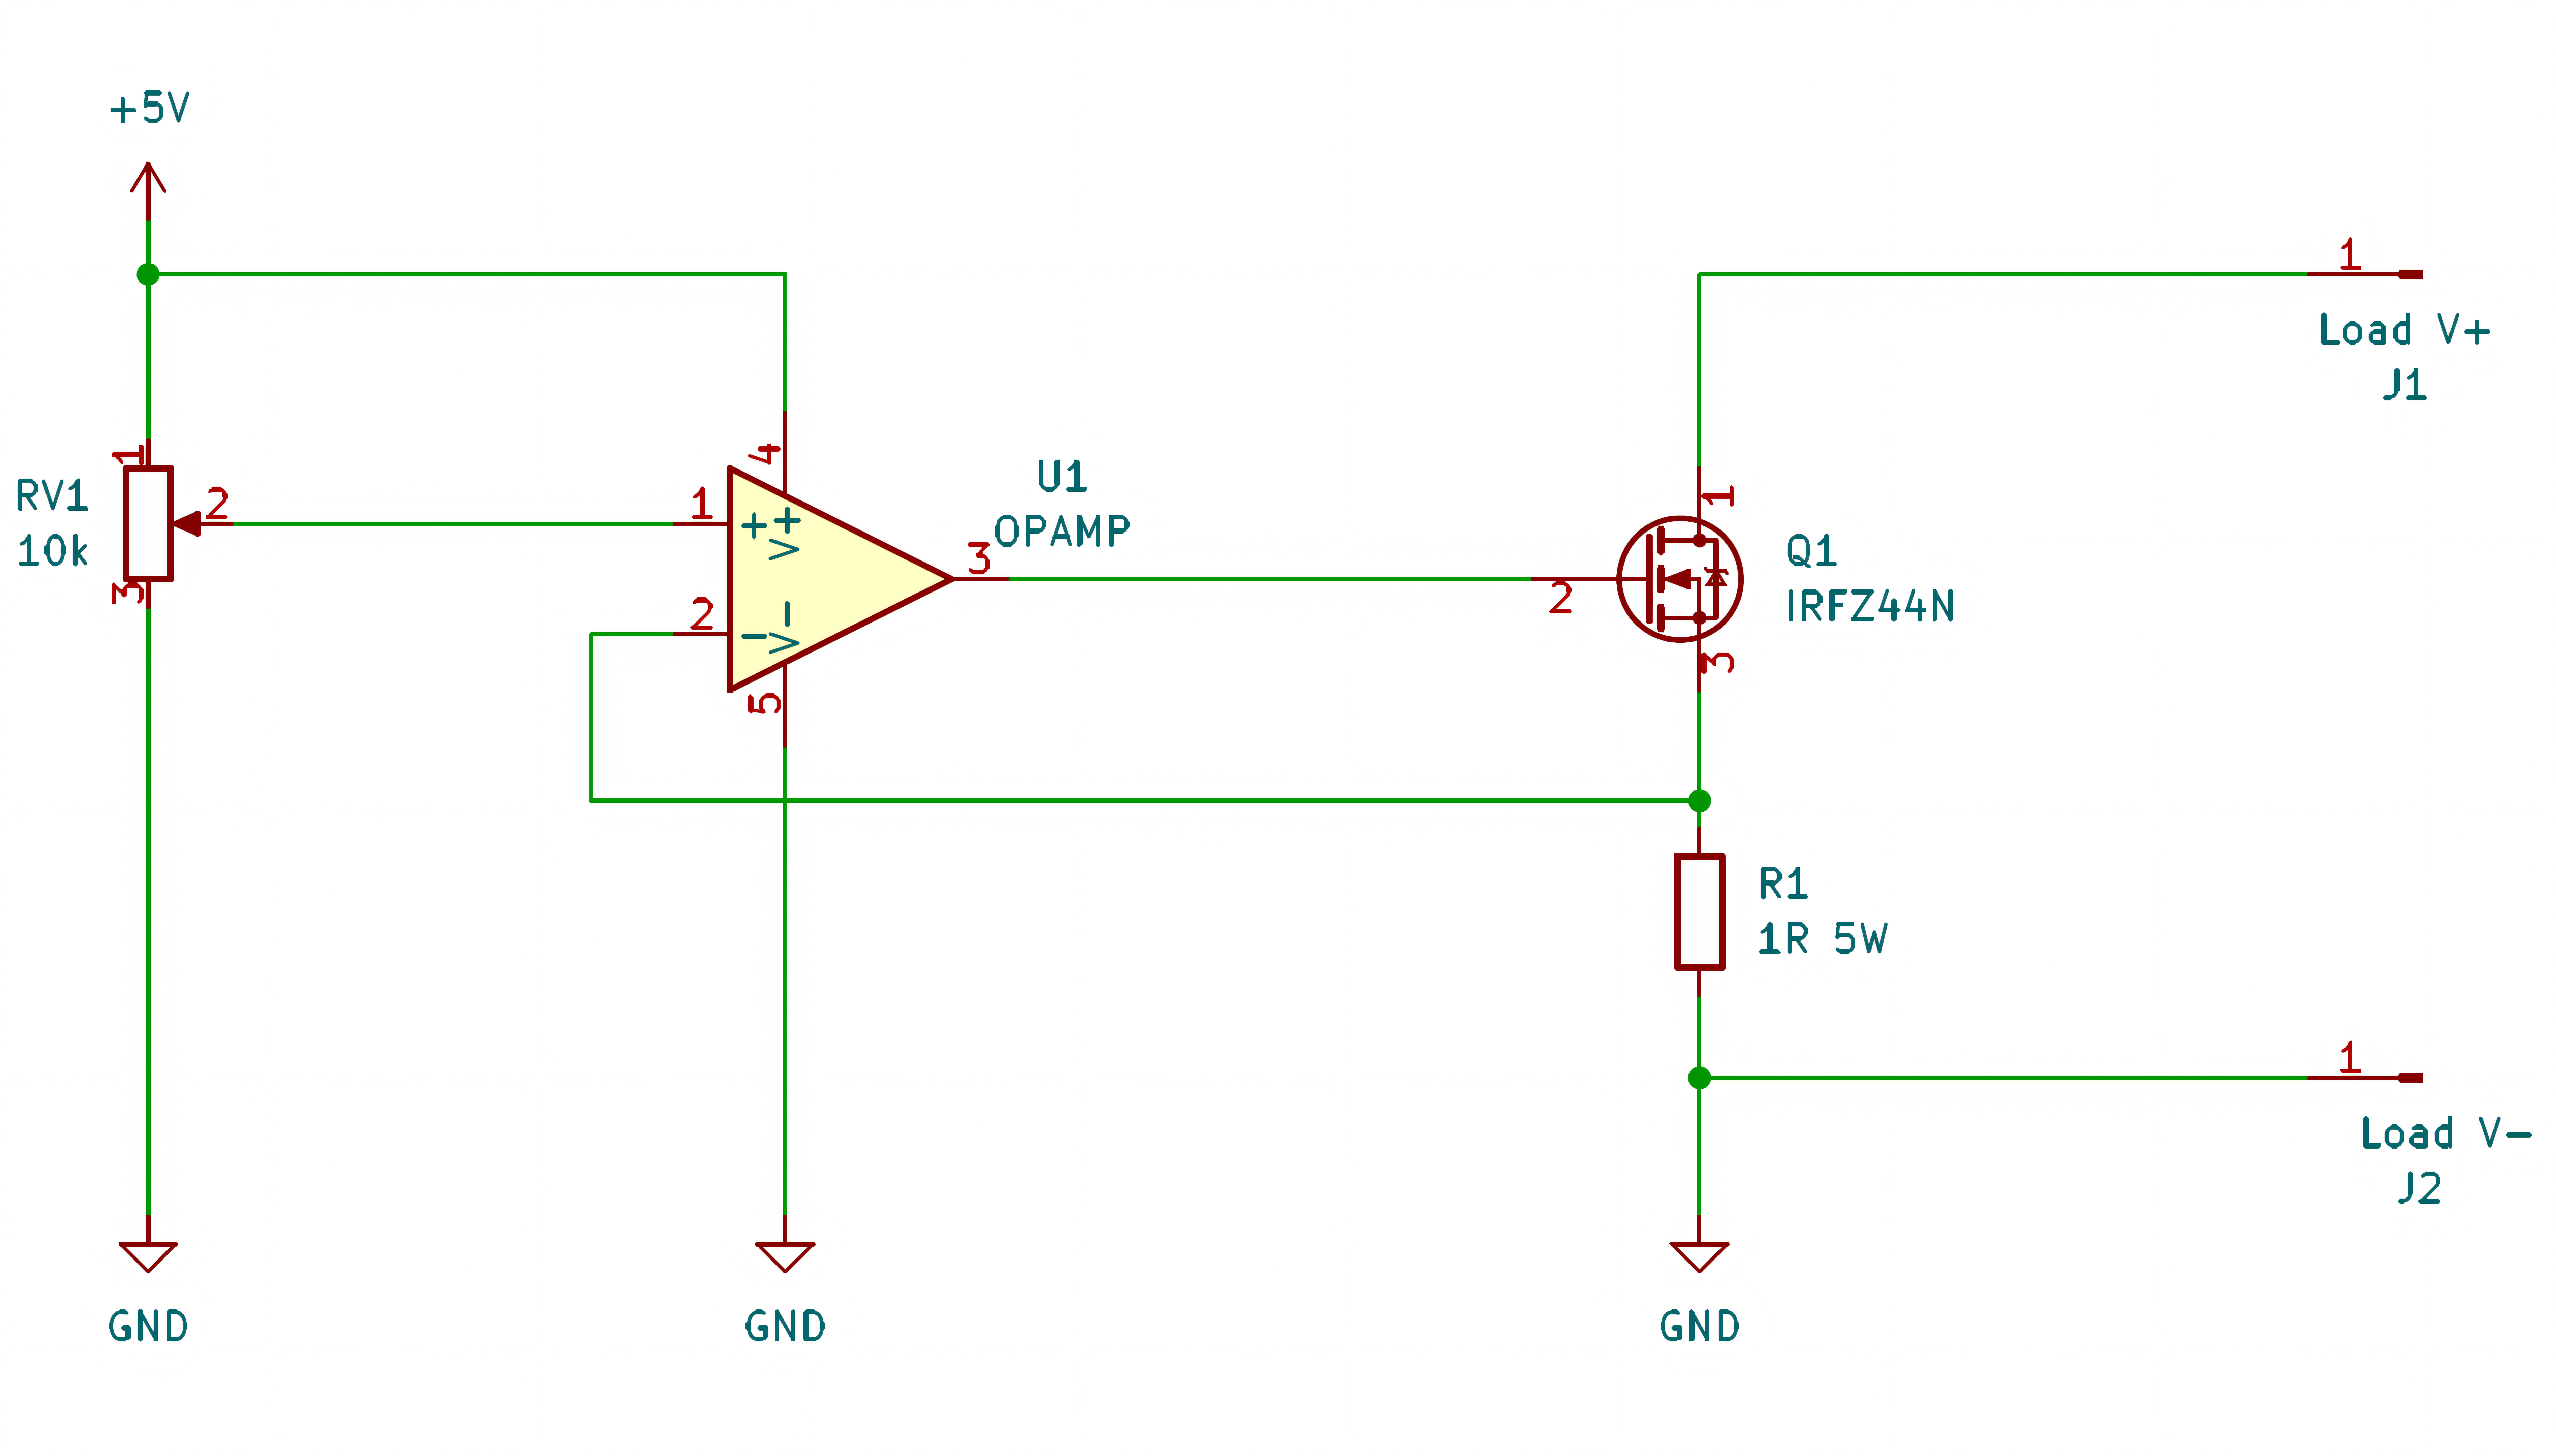
\includegraphics[width=\columnwidth]{IMGS/LoadSchematic.jpg}
	\caption{Variable DC load schematics}
	\label{fig:arch}
\end{figure} 
\\ \\	
\section{Testing of DC/DC converters}
DC/DC converters have a specified input voltage operating range. To confirm the DC/DC converter works properly over the entire range of input voltages, they are tested using an adjustable or programmable dc source to provide the input voltage. A dc electronic load is used on the output of the DC/DC converter to set the output load current and simulate the device that the DC/DC converter would power.

\subsection{Input turn-on, input turn-off voltage levels and timing test}

To test the minimum input voltage turn-on level, the DC/DC converter is turned on using the nominal input voltage while using the electronic load to apply the maximum rated output current or power. The input voltage is then reduced until the unit output begins to drop or the minimum input voltage setting is met.
\\ \\
To confirm the DC/DC converter would turn on with a maximum load on the output, the input voltage would be set to the minimum and toggled off and back on while measuring the output voltage and current. The output voltage and ripple and noise may also be measured to see if the lower input voltage setting has any effect on the output stability or ripple.
\\ \\
Additionally, this setup can be used to test and measure the turn-on time, turn-off time, and hold-up times. An oscilloscope is used for the ripple and for periodic and random deviation (PARD) measurements.
\\ \\
\begin{figure}[h]
	\centering
	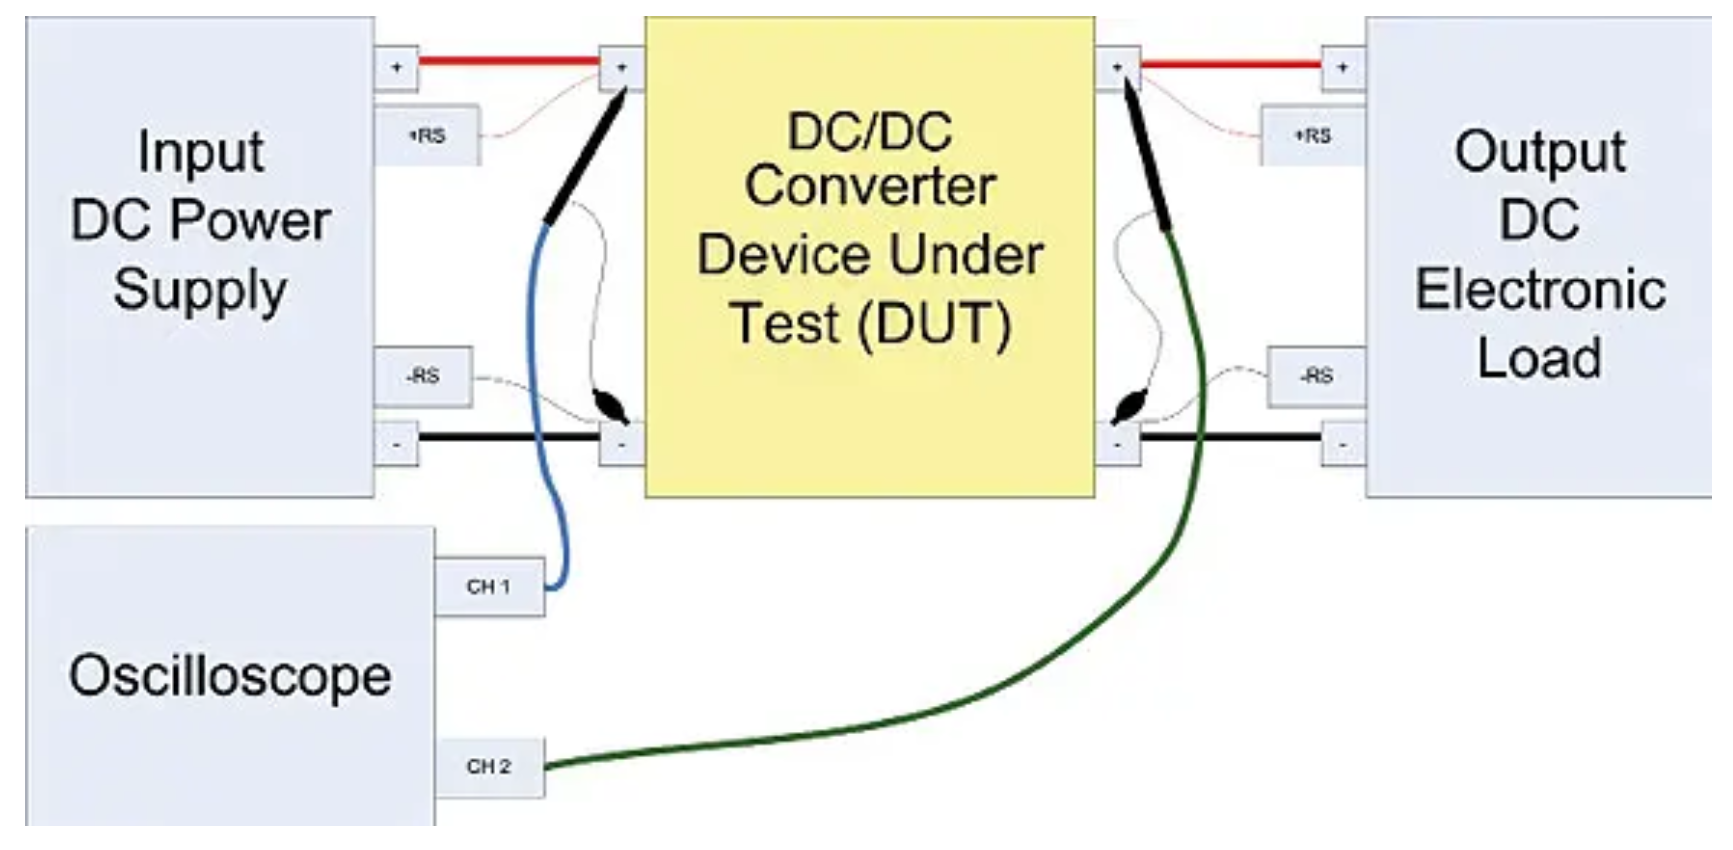
\includegraphics[width=\columnwidth]{IMGS/DCDCconverterTestSetup.jpg}
	\caption{Test setup}
	\label{fig:arch}
\end{figure} 
\\ \\	
Turn-on time indicates the period from the time at which the minimum input voltage is applied to the time the output voltage is within the output regulation limits. Turn-off time indicates when the input voltage drops below the specified minimum and the output turns off or drops to zero volts.
\\ \\
\begin{figure}[h]
	\centering
	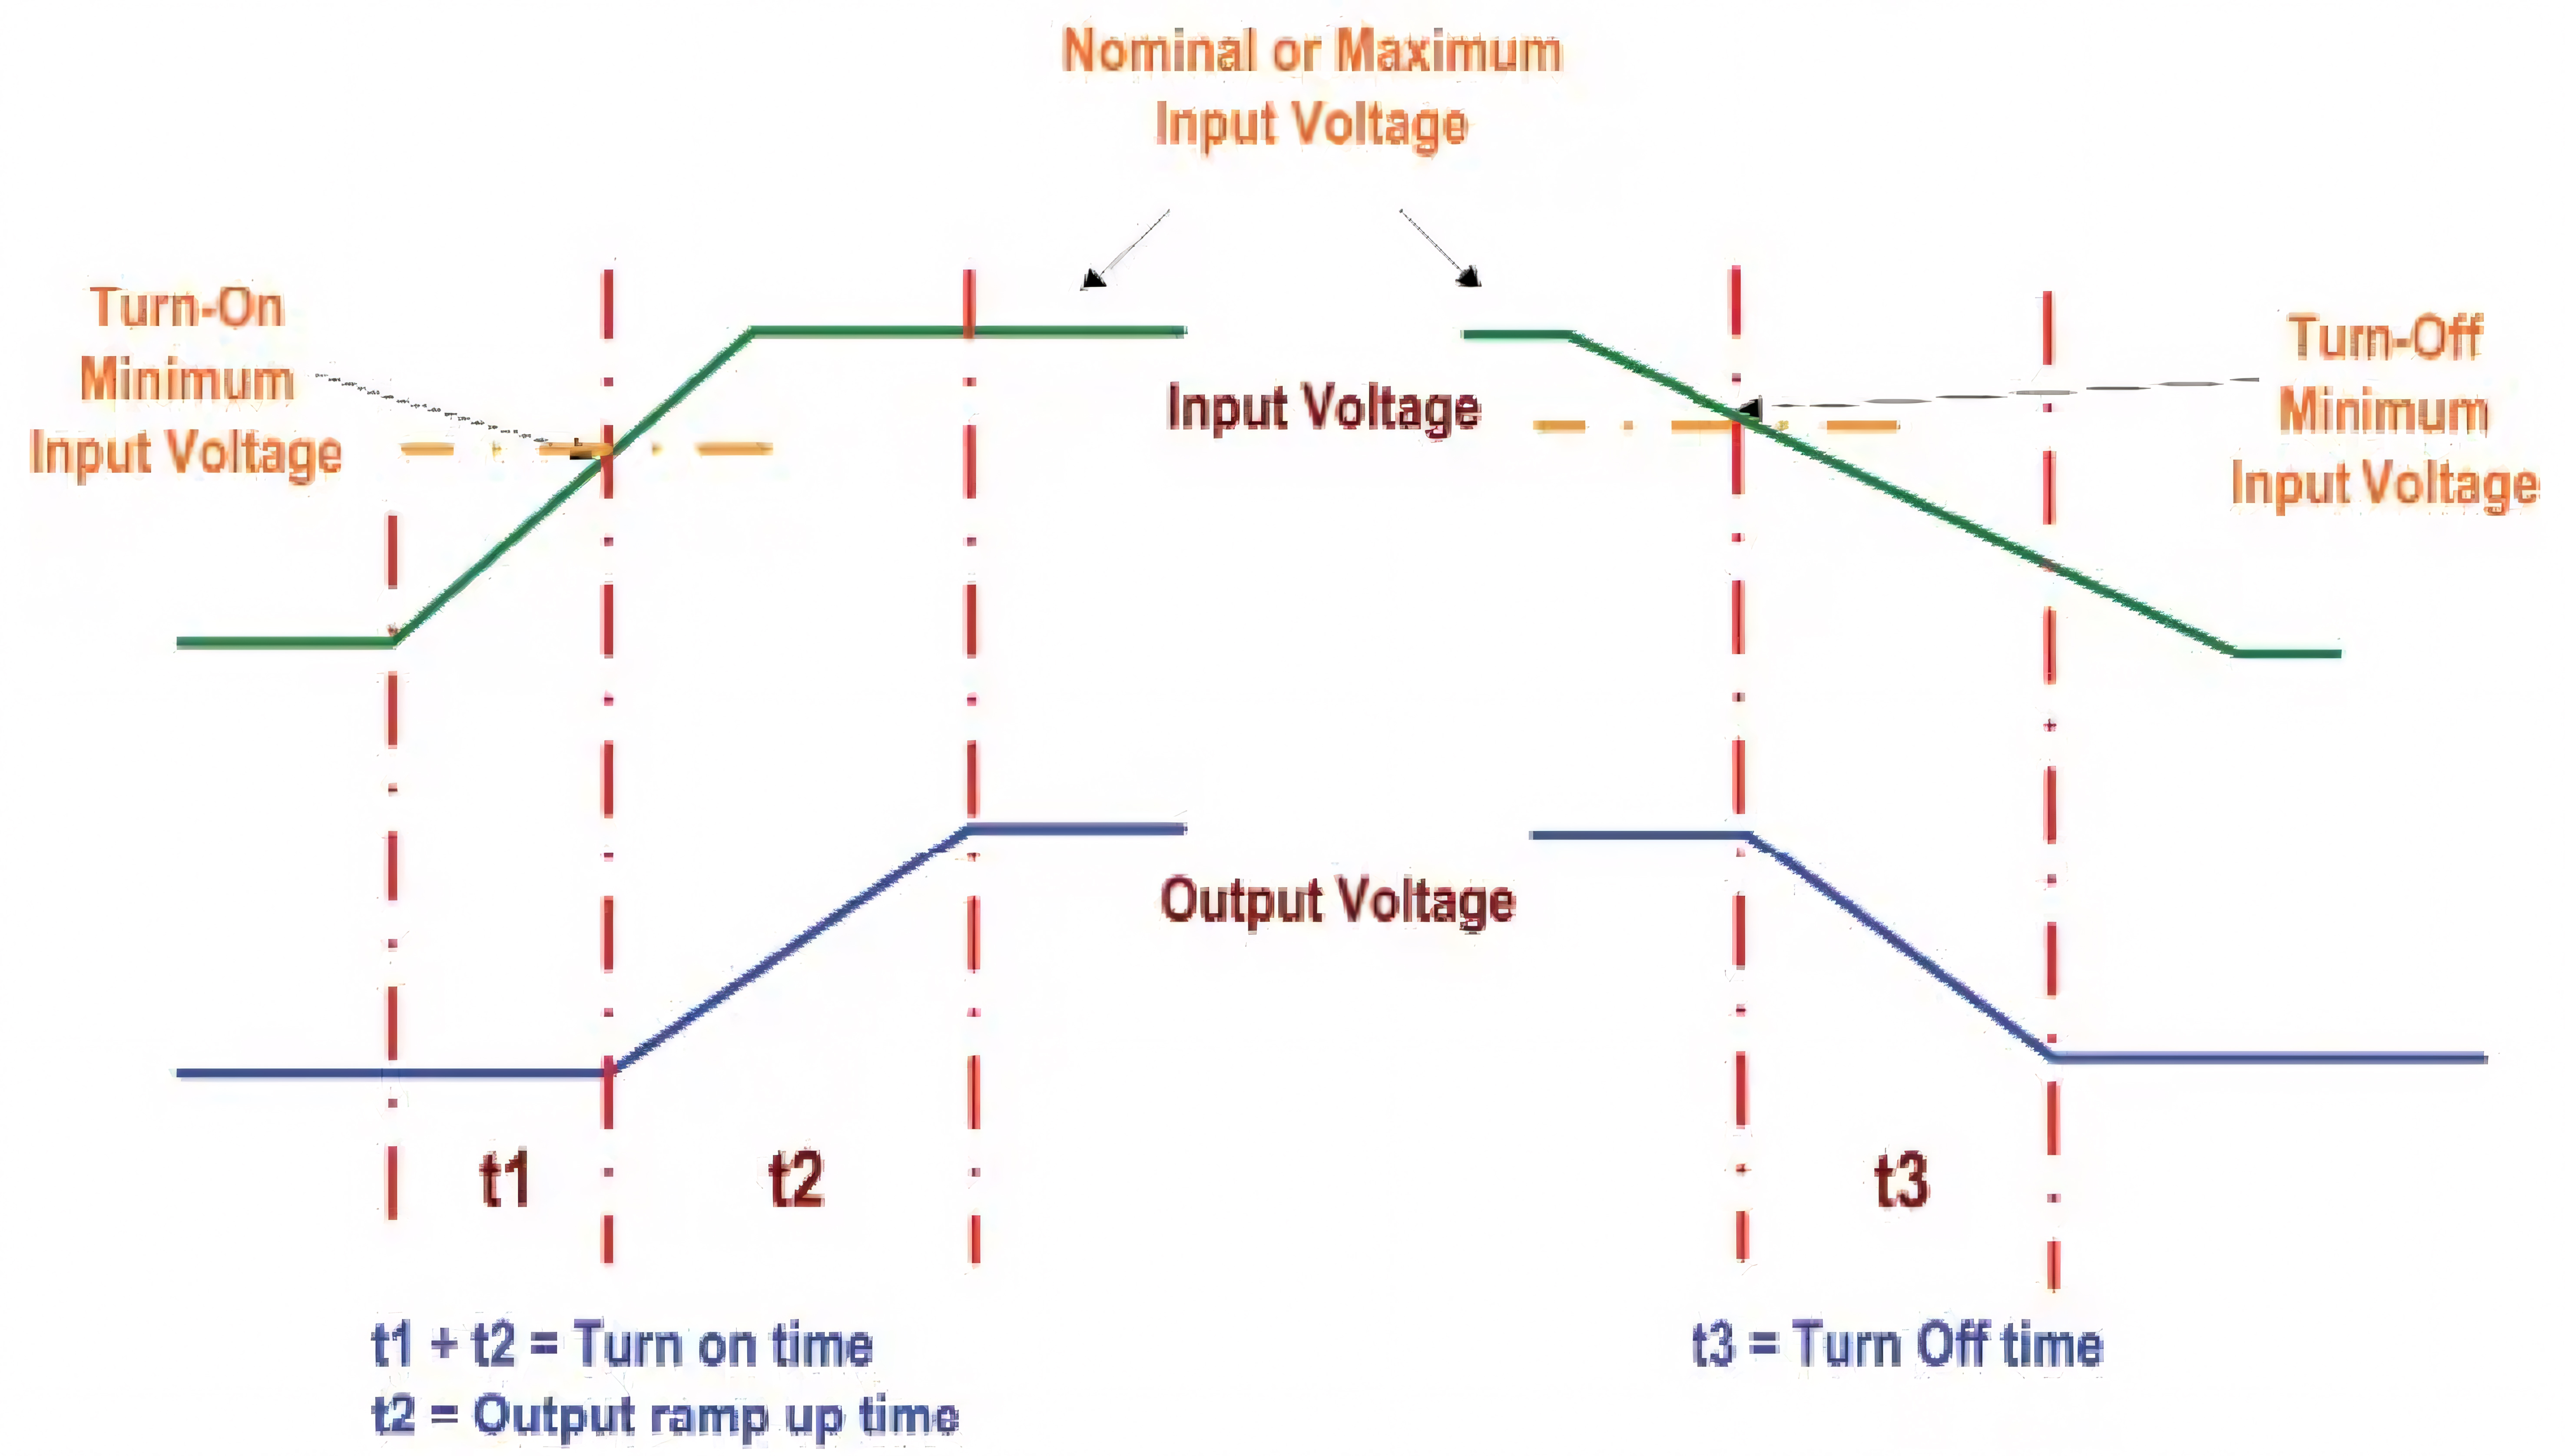
\includegraphics[width=\columnwidth]{IMGS/TurnOnTurnOff.jpg}
	\caption{Turn-on, Turn-off characteristics}
	\label{fig:arch}
\end{figure} 
\\ \\	
The hold-up timing test can use the same setup as the input turn-on and turn-off test. Hold-up timing indicates the time from when the input drops below the minimum input voltage and the output voltage drops below its minimum regulated output tolerance. This test also indicates how well the output of the DC/DC converter can continue to operate despite short interrupts and drops in the input voltage. Some DC/DC converters have an input fault detection signal. If so, this signal can be used to trigger the test.
\\ \\
\begin{figure}[h]
	\centering
	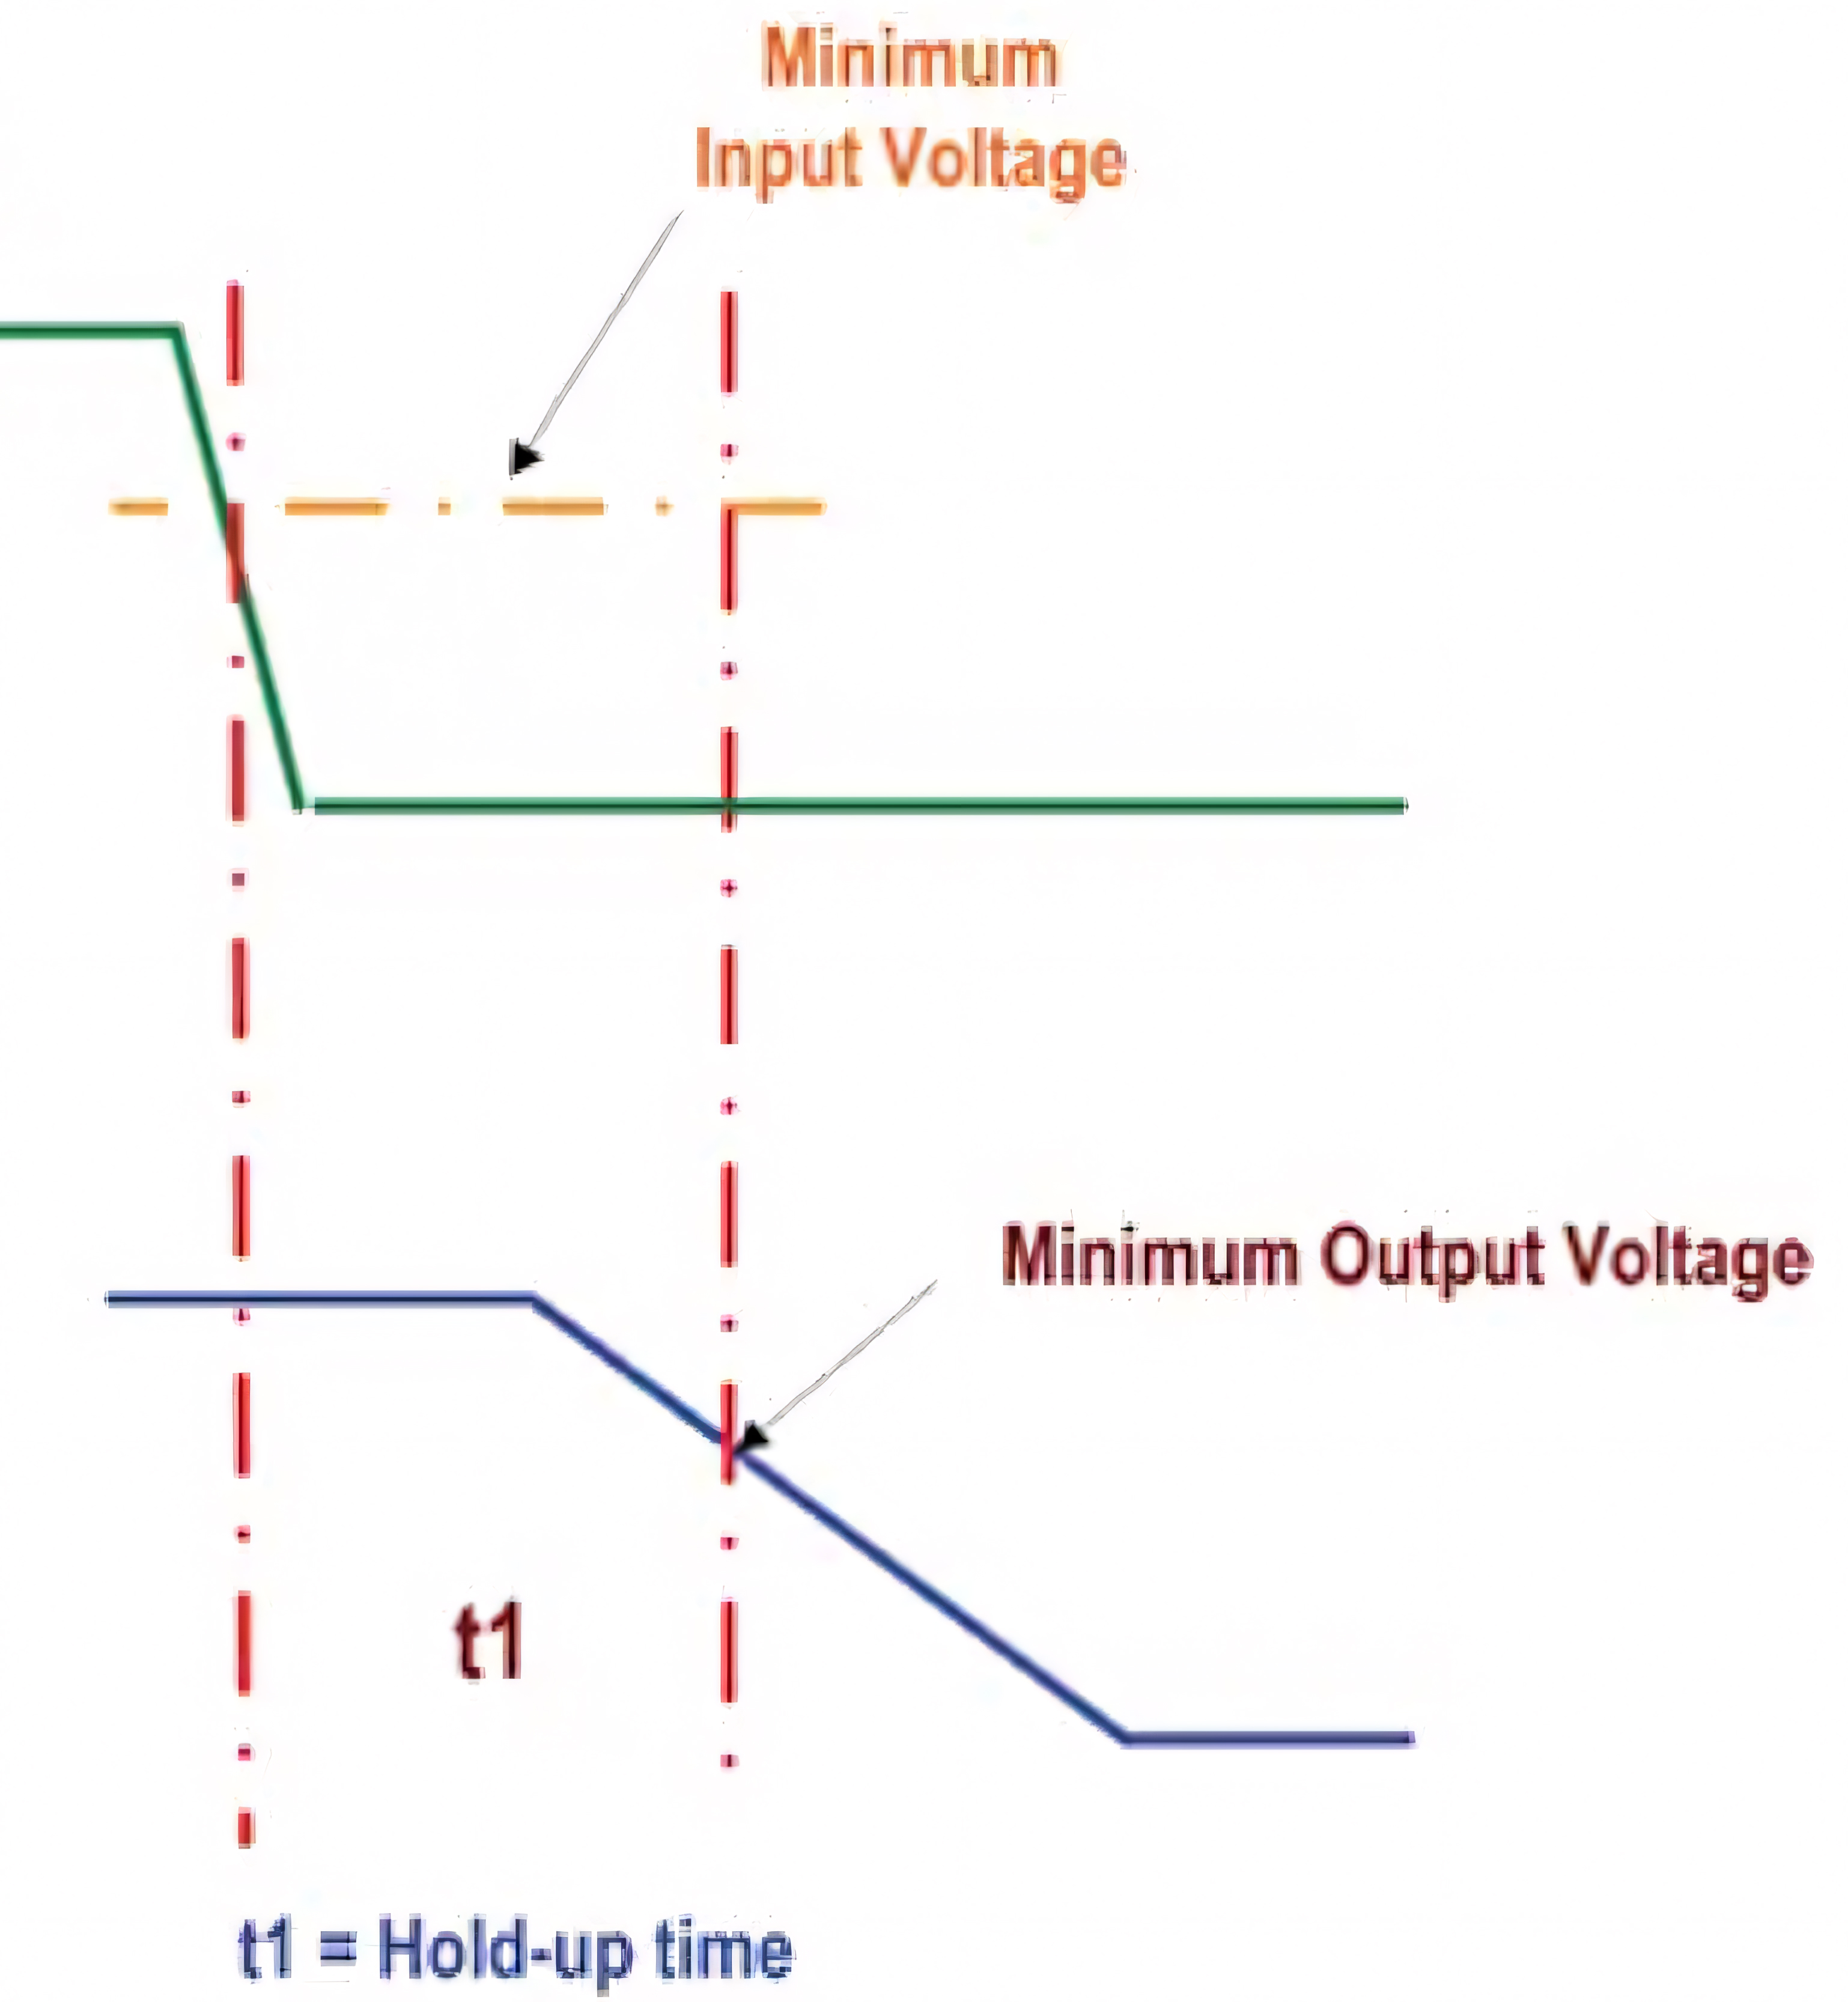
\includegraphics[width=140pt]{IMGS/HoldUpTimeTest.jpg}
	\caption{Hold-up time characteristics}
	\label{fig:arch}
\end{figure} 
\\ \\
\subsection{Output line regulation}

This test confirms that the output voltage stays within specified regulation limits when the input voltage varies from minimum to maximum operating voltage, as defined in the DC/DC converter specification. During this test the output load is usually set to nominal or maximum current as specified.
\\ \\
The output line regulation test involves monitoring the output voltage and recording the total voltage deviation while varying the input voltage from its minimum to maximum specified limits. Some specifications show the output tolerance as a voltage (i.e. 3.3 Vdc ± 0.02 V) or as a percentage (i.e. 3.3 V ± 0.5\%).
\\ \\
Output regulation $R_{o}$ is calculated as a percentage and given by the equation:
\\ \\
\hspace*{5cm}$R_{o}$ = $\left | \frac{V_{omax}-V_{omin}}{V_{onom}} \right | \times 100$
\\ \\
where:
$V_{omax}$ = Vout at Vin max; 
$V_{omin}$ = Vout at Vin min; and
$V_{onom}$ = Vout nominal.
\\ \\
\subsection{Output load regulation} 
The output load regulation test ensures the DC/DC converter output voltage stays within the specified regulation tolerance. Here, the change in output voltage is recorded while load is varied from minimum to maximum current. This delta voltage is used to calculate the percentage of deviation which is compared to the specified load regulation limits. Load regulation $L_{r}$ is calculated as a percentage from the equation:
\\ \\
\hspace*{5cm}$L_{r}$ = $\left | \frac{V_{oio}-V_{oim}}{V_{onom}} \right | \times 100$
\\ \\
where:
$V_{oio}$ = Vout at Iout max; 
$V_{oim}$ = Vout at Iout min; and
$V_{onom}$ = Vout nominal.
\\ \\
\subsection{Output transient response deviation and time}

 This test determines how well the output voltage responds to a sudden change in output current. The measurement includes the maximum output voltage deviation and the time it takes for the voltage to recover to its regulated output nominal voltage tolerance.
\\ \\
For this test, a dc electronic load is set for a minimum and maximum current and then set for the slew rate for the rising and falling edge of the current transition. The frequency and duty cycle can also be set for the pulsed current.
\\ \\
\subsection{Output ripple and noise voltage} 

The output ripple and PARD reflects the output voltage of the DC/DC converter and its ability to filter out ripple and noise. Various topologies used in DC/DC converters have different internal switching frequencies which are reflected in the output ripple frequency. For example, internal chopper circuit transients can generate higher frequency noise. The output noise and ripple are measured using an oscilloscope. To avoid erroneous noise, it is important to minimize the length of the ground wire on the voltage probe.
\\ \\
\subsection{Output over-current protection}

The output over-current protection is intended to protect the DC/DC converter and the device it powers when the load exceeds the converter’s maximum rated current. There are different methods used in over-current protection. But the typical approaches are fold-back current limit and pulsing current-limit. The latter is generally referred to as hiccup-mode current limit.
\\ \\
Here are the differences between the two methods: In fold-back current limiting, the output voltage begins to drop and limits the output current supplied to the load as the load current rises above the current-limit set point. In hiccup current limiting, the output turns off when the output current exceeds the rated current limit point. It eventually turns back on. If the load continues to exceed the current-limit set-point, the output will continue turning on and off, hence the hiccup-mode name.
\\ \\
\subsection{Output over-voltage protection} 

Most DC/DC converters have a built-in protection circuit that will shut off the output of the device when the output voltage is detected to be over the maximum limit. This facility is referred to as over-voltage protection (OVP). This protects the DC/DC converter from external excessive voltage applied to the converter output. If the DC/DC converter has an adjustable output (trimmed or programmable output voltage), it may be possible to increase the output voltage until the OVP point is exceeded and the protection circuit activates.
\\ \\
If the DC/DC converter does not have an adjustable output, an external voltage source can be applied across the output terminal, increased to the OVP trip point, then removed to see if the output has triggered and turned off.
\\ \\
DC/DC converters having an OVP fault signal can use it to determine if the output detected the OVP and, if so, shut off the output. The output voltage is monitored to determine when the OVP happened and then compared to the OVP specified limits.
\\ \\
\subsection{Output operating temperature and over-temperature protection} 

DC/DC converters have an operating temperature range, and many have an over-temperature protection (OTP) circuit that will turn off the output if temperature gets sufficiently high. For this test, a thermal chamber can raise and lower the DC/DC converter temperature to simulate the operating temperature range.
\\ \\
Thermocouples and thermal probes or infrared thermal measurement devices can measure the temperatures on the body of the DC/DC converter. During the operating temperature test, the DC/DC converter is loaded to its maximum rating for current and power. Meanwhile, the output voltage is monitored to verify it stays within specified limits.
\\ \\
During the test, the device temperature is recorded while monitoring the output voltage until the OTP circuit triggers and the output shuts off. The unit is then allowed to cool and input voltage is toggled off and on to verify the DC/DC converter recovers from the OTP.
\\ \\
\subsection{Efficiency} 

Efficiency determines the internal power dissipated by the DC/DC converter and how efficiently input power transfers to the converter output. This test usually takes place at the nominal input voltage and with the output load set to nominal or maximum specified ratings. The input voltage, current, and power is measured while the same parameters are measured on the output. Efficiency percentage $E_{p}$ comes from the equation:
\\ \\
\hspace*{5cm}$E_{p}$ = $\left | \frac{V_{out}-I_{out}}{V_{in}-I_{in}} \right | \times 100$
\\ \\
where:
Vout and Iout = converter output voltage and current;
Vin and Iin = converter input voltage and current.
\\ \\
This test can also capture the efficiency at various power levels. It’s common to plot the data to show efficiency versus output-current.

\section{Battery Charger Testing}



	







